% 劳埃德镜实验
% 劳埃德镜|干涉|光密介质

\pentry{杨氏双缝干涉实验\upref{Young}, 半波损失\upref{WvLost}}

劳埃德(H.Lloyd)于1834年提出了一种更简单的观察干涉的装置.如\autoref{Lloyd_fig1}所示,$MN $为一块平玻璃板,用作反射镜,$S_1$是一狭缝光源,从光源发出的光波,一部分掠射(即入射角接近$90^\circ$)到玻璃平板上,经玻璃表面反射到达屏上;另一部分直接射到屏上.这两部分光也是相干光,它们同样是用分波阵面得到的.反射光可看成是由虚光源$S_2 $发出的.$S_1$和$S_2 $构成一对相干光源,对干涉条纹的分析与杨氏实验也相同.中画有阴影的区域表示相干光在空间叠加的区域.这时在屏上可以观察到明暗相间的干涉条纹.
\begin{figure}[ht]
\centering
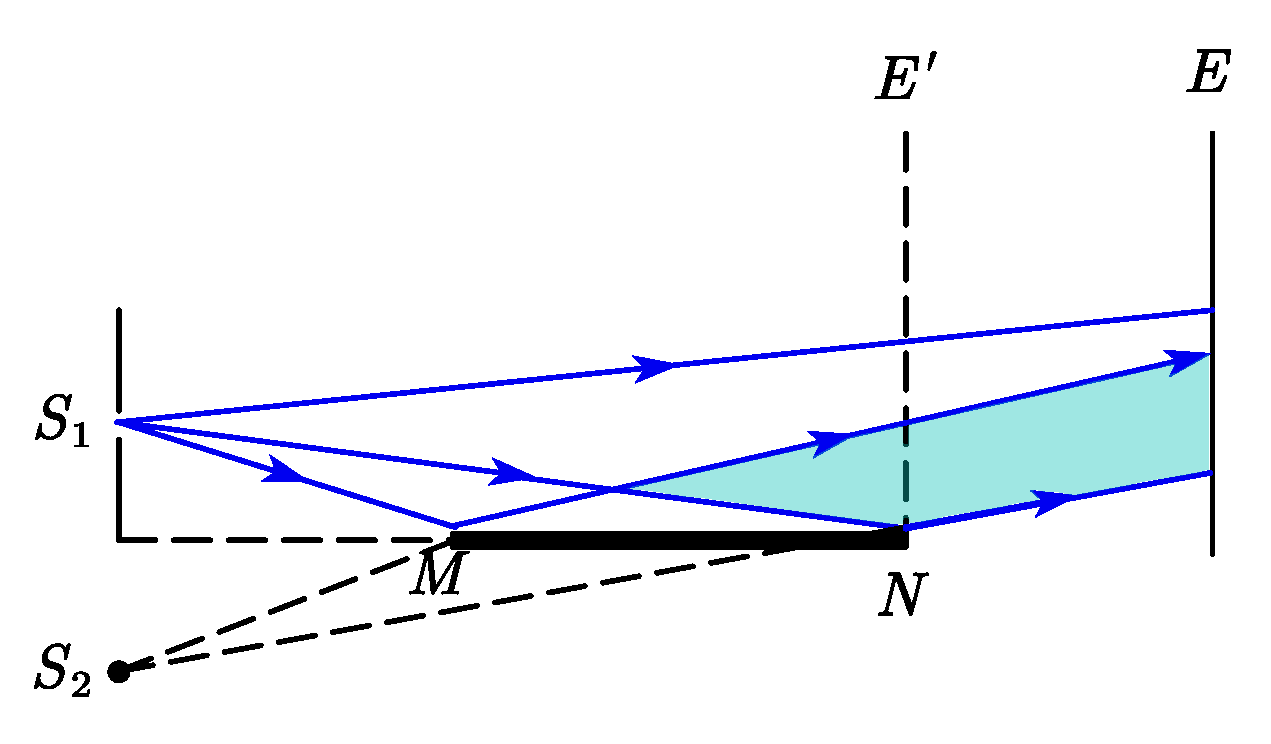
\includegraphics[width=8cm]{./figures/Lloyd_1.pdf}
\caption{劳埃德镜实验} \label{Lloyd_fig1}
\end{figure}
应该指出,在劳埃德镜实验中,如果把屏幕移近到和镜面边缘$N $相接触,即\autoref{Lloyd_fig1}中$E' $的位置,这时从$S_1$和$S_2$发出的光到达接触处的路程相等,应该出现明纹,但实验结果却是暗纹,其他的条纹也有相应变化.这一实验事实说明了由镜面反射出来的光和直接射到屏上的光在$N $处的相位相反,即相位差为$\pi$. 由于直射光的相位不会变化,所以只能认为光从空气射向玻璃平板发生反射时,反射光的相位跃变了$\pi$.

进一步的实验表明: 光从光疏介质射到光密介质界面反射时,在掠射(入射角$i=90^\circ$或正入射,即$i = 0$)的情况下,反射光的相位较之入射光的相位有$\pi$的突变,这一变化导致了反射光的波程在反射过程中附加了半个波长,故常称为\textbf{半波损失}.今后在讨论光波叠加时,若有半波损失,在计算波程差时必须计及,否则会得出与实际情况不符的结果.
